\documentclass[11pt]{beamer}
\author{Philipp Arras, Florian Nowak}
\title{\LaTeX -Kurs}
\date{11. Oktober 2014}

\usetheme{Berkeley}
%\setbeamercovered{transparent}
\setbeamertemplate{navigation symbols}{}
%\logo{}
%\institute{}
%\subject{}

\usepackage[utf8]{inputenc}
\usepackage[ngerman]{babel}
\usepackage{amsmath,amsfonts,amssymb}
\usepackage{graphicx,booktabs}

\usepackage{pdfpages}

\begin{document}

%\begin{frame}
%\titlepage
%\end{frame}

%\begin{frame}
%\tableofcontents
%\end{frame}

\section{Einleitung}
\begin{frame}{Was genau ist überhaupt dieses {\LaTeX}?}
\textbf{Aus Wikipedia:}

\smallskip
\begin{itemize}
\item \textbf{\TeX} ist ein von \textbf{Donald E. Knuth} ab 1977 entwickeltes und 1986 fertiggestelltes Textsatzsystem mit eingebauter Makrosprache (die ebenfalls {\TeX} genannt wird).
\item \textbf{\LaTeX} ist ein Softwarepaket, das die Benutzung des Textsatzsystems {\TeX} mithilfe von Makros vereinfacht;\\
es liegt derzeit in der Version $2_\varepsilon$ vor.
\end{itemize}
\end{frame}

\begin{frame}{Der Urvater}
\textbf{Wieder aus Wikipedia:}

\medskip\noindent
\textbf{Donald Ervin {\glqq}Don{\grqq} Knuth} (geboren am 10. Januar 1938) ist ein US-amerikanischer Informatiker, emeritierter Professor an der Stanford University und Autor des mehrbändigen Standardwerks \textit{The Art of Computer Programming} (für dessen Textsatz er eigens die Programme {\TeX} und METAFONT entwickelt hat). 
\end{frame}

\begin{frame}{Der Urvater}
\begin{figure}
\centering
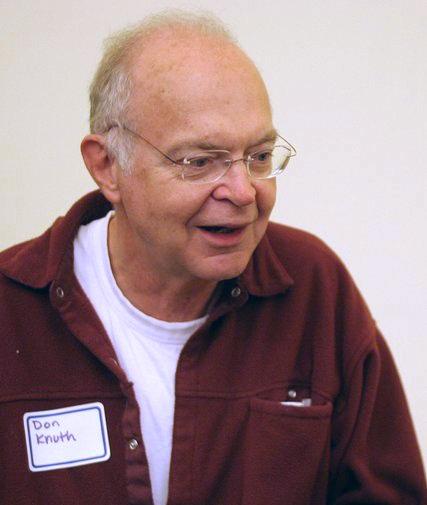
\includegraphics[scale=.45]{KnuthAtOpenContentAlliance}
\caption{Donald Knuth (2005)}
\end{figure}
\end{frame}

\begin{frame}{Erweiterungen von {\TeX}}
\begin{itemize}
\item \textbf{pdfTeX:} Erweiterung von {\TeX}, mit der aus {\TeX}- sowie {\LaTeX}-Quellen unmittelbar \textbf{PDF}-Dateien erzeugt werden können (PDF hat zunehmend die {\glqq}alten{\grqq} {\TeX}-Ausgabeformate DVI und PostScript verdrängt)
\item \textbf{LuaTeX:} Nachfolger von pdfTeX (aktuell in der stable beta 0.79.1), der über die darin eingebettete Skriptsprache \textbf{Lua} gesteuert werden kann; die standardmäßige Eingabekodierung ist \textbf{Unicode}
\end{itemize}
\end{frame}

{
\setbeamercolor{background canvas}{bg=}

\includepdf[pages={35-37,27}]{01-Einfuehrung}
}

\begin{frame}{Installation und Editoren}
\textbf{Installation über}

\smallskip
\begin{itemize}
\item \textbf{TeX Live} (\url{http://www.tug.org/texlive/})\\
(Version von 2013 ist auf den URZ-Rechnern installiert)
\item MiKTeX oder proTeXt (Windows)
\item MacTeX
\end{itemize}
\end{frame}

\begin{frame}{Installation und Editoren}
\textbf{Installation über}

\smallskip
\begin{itemize}
\item \textbf{TeX Live} (\url{http://www.tug.org/texlive/})\\
\item MiKTeX oder proTeXt (Windows)
\item MacTeX
\end{itemize}

\smallskip\noindent
\textcolor{red}{! Wir empfehlen eine \emph{vollständige} (aktuelle) Installation von TeX Live !}
\end{frame}

\begin{frame}{Installation und Editoren}
\textbf{Editoren:}

\smallskip
\begin{itemize}
\item Bei der Installation von TeX Live kann \textbf{TeXworks} mitinstalliert werden
\item \textbf{Texmaker} (praktisch wegen Befehlsvervollständigung über Tab-Taste und Rechtschreibprüfung/Wörterbüchern)
\item Andere, z. B. Sublime Text
\end{itemize}
\end{frame}

\begin{frame}{Erste Beispiele}
\emph{(Beispiele vorführen!)}
\end{frame}

\end{document}